\section{Future Work}

\subsection{Expand Library of Primitives}
In this paper we have made many simplifications to the problem space just to make the placer easier to implement.
For example, our placer in its current state does not take advantage of \texttt{SLICEL}/\texttt{SLICEM} homogeneity and simply maps all SLICE \texttt{SiteInst}s onto \texttt{SLICEL}s. 
Recall that the SLICE Sites in Xilinx FPGAs typically come in a 75-25\% split between \texttt{SLICEL}s and \texttt{SLICEM}s. 
This means that we have rendered about 25\% of the CLB fabric unusable which will inevitably hurt wirelength minimization during placement since the \texttt{SiteInst}s must be spread over a larger area. 
Enabling \texttt{SLICEL}-\texttt{SLICEM} homogeneity can lead do greater logic density and consequently less total HPWL, but can make the packing process more complex and may contribute to higher routing congestion.

\subsection{Robustness}
In its current state, the prepacker and packer struggle with data busses larger than 24-bits, especially with DSP functions like multiplication. 
In such designs, the synthesizer will synthesize \texttt{CARRY4} chains with particular \texttt{EDIFHierPortInst} configurations that are currently not supported by our packer which eventually lead to errors or failures in the subsequent routing stage.
Further work is required to resolve these routing constraints.

\subsection{Improvements to Packing}
There is also no rule saying we must pack \texttt{Cells} into \texttt{SiteInst}s before placement or that we follow a strict prepacking-packing-placement flow. 

Our current pack-place approach is a \texttt{Site}-centric approach and resembles that of Xilinx ISE, which is the predecessor to the Vivado design suite.
The latest editions of Vivado performs BEL-centric placement without necessarily locking \texttt{Cell}s into \texttt{Site}s, allowing a higher granularity of movement of \texttt{Cell}s during placement. 

{
    \centering
    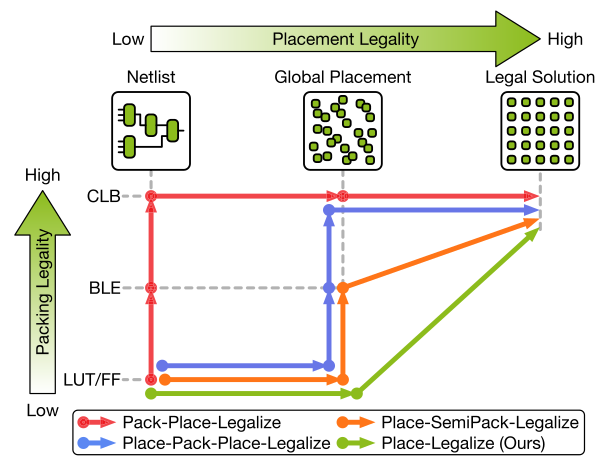
\includegraphics[width=\columnwidth]{figures/future_work/legalization.png}
    \captionof{figure}{Representative FPGA placement and packing flows. Figure taken from Wuxi et al. (2019), page 1 \cite{ExplicitPacking}}
}
\vspace{0.25cm}



\subsection{Improvements to SA}

\subsection{Force-Directed and Analytical Placement}




